\section{Run-Time Assurance}

[DARREN - 1.5 pg]

Run-Time Assurance Architecture -- ASTM F3269-17 standard [DARREN]

Run-time assurance architectures add high-assurance components
to the system to ensure that an LEC cannot cause
unsafe or unintended system behaviors. Run-time monitors
continuously check variables related to the system state, inputs
to the LEC, or outputs produced by the LEC and intervene to
switch to a backup function that is proven to be safe. Monitors
may be used to detect anomalous inputs that are outside of the
data distribution used to train the system and therefore could
lead to unintended behavior. The main idea is that system
performance is provided by the LEC while system safety is
guaranteed by high-assurance components (though with lower
performance).

In the DARPA Assured Autonomy project we have used a
run-time assurance architecture based on the ASTM F3269-17
standard for bounded behavior of complex systems \cite{F3269-17}, also
known as a simplex architecture \cite{simplex}. The standard provides
guidance for mitigating unintended functionality through the
use of run-time monitors. The LEC may still contain unintended
functionality, but the architecture ensures that there will
be no impact on system safety. This approach essentially uses
the verified properties of the architecture, run-time monitor,
and safety backup functions to justify a reduced level of
criticality for the LEC.

Monitors, high-assurance components, backup avoidance plan

Run-time assurance architecture was developed to guarantee the absence of unintended behavior resulting from the collision avoidance neural network

- RTA, AADL model [DARREN/ISAAC]

- Trajectory prediction, SWC assessment [RAM/DARREN]


\begin{figure*}
	\centering
	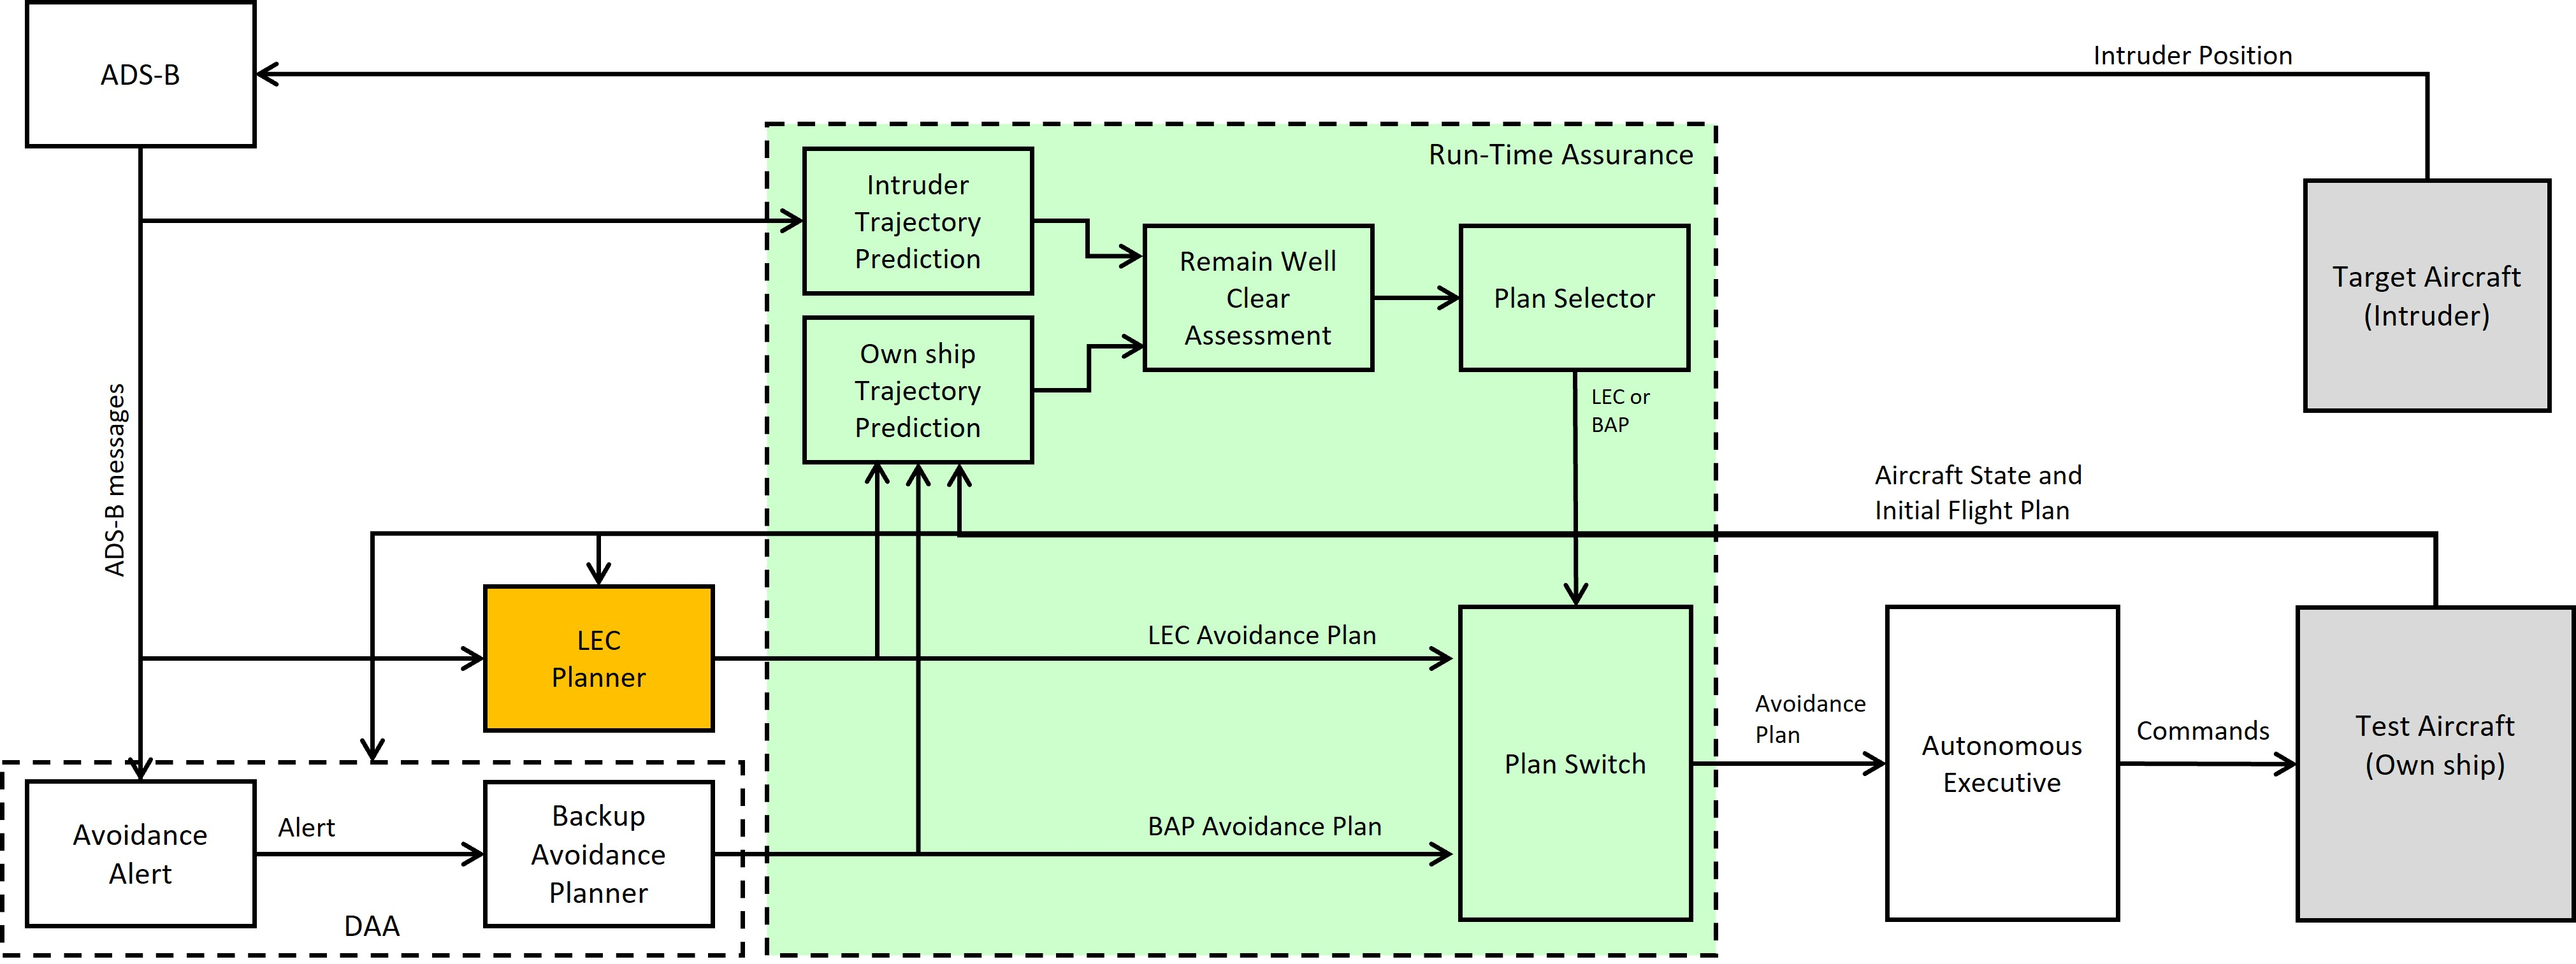
\includegraphics[width=\textwidth]{figures/rta-arch.jpg}
	\caption{Run-Time Assurance Architecture}
	\label{fig:rta-arch}
\end{figure*}

